\chapter{Implementation}

In this chapter, take a look at how the GoDeliver system works and the integration of the \gls{vrptw} \gls{ai} planner.

\section{GoDeliver System}

The GoDeliver system is consisted of multiple services, each responsible for a given subproblem of the delivery process. The core of the system is GoDeliver service, which implements all system APIs and performs the basic CRUD operation on our NoSQL database. The database stores information about business, delivery orders, couriers, and delivery plans. In the Figure \ref{fig:godeliver-system} is visualized the simplified architecture of GoDeliver system, it is especially oriented to show how the planning process works.

\begin{figure}[ht]
    \centering
    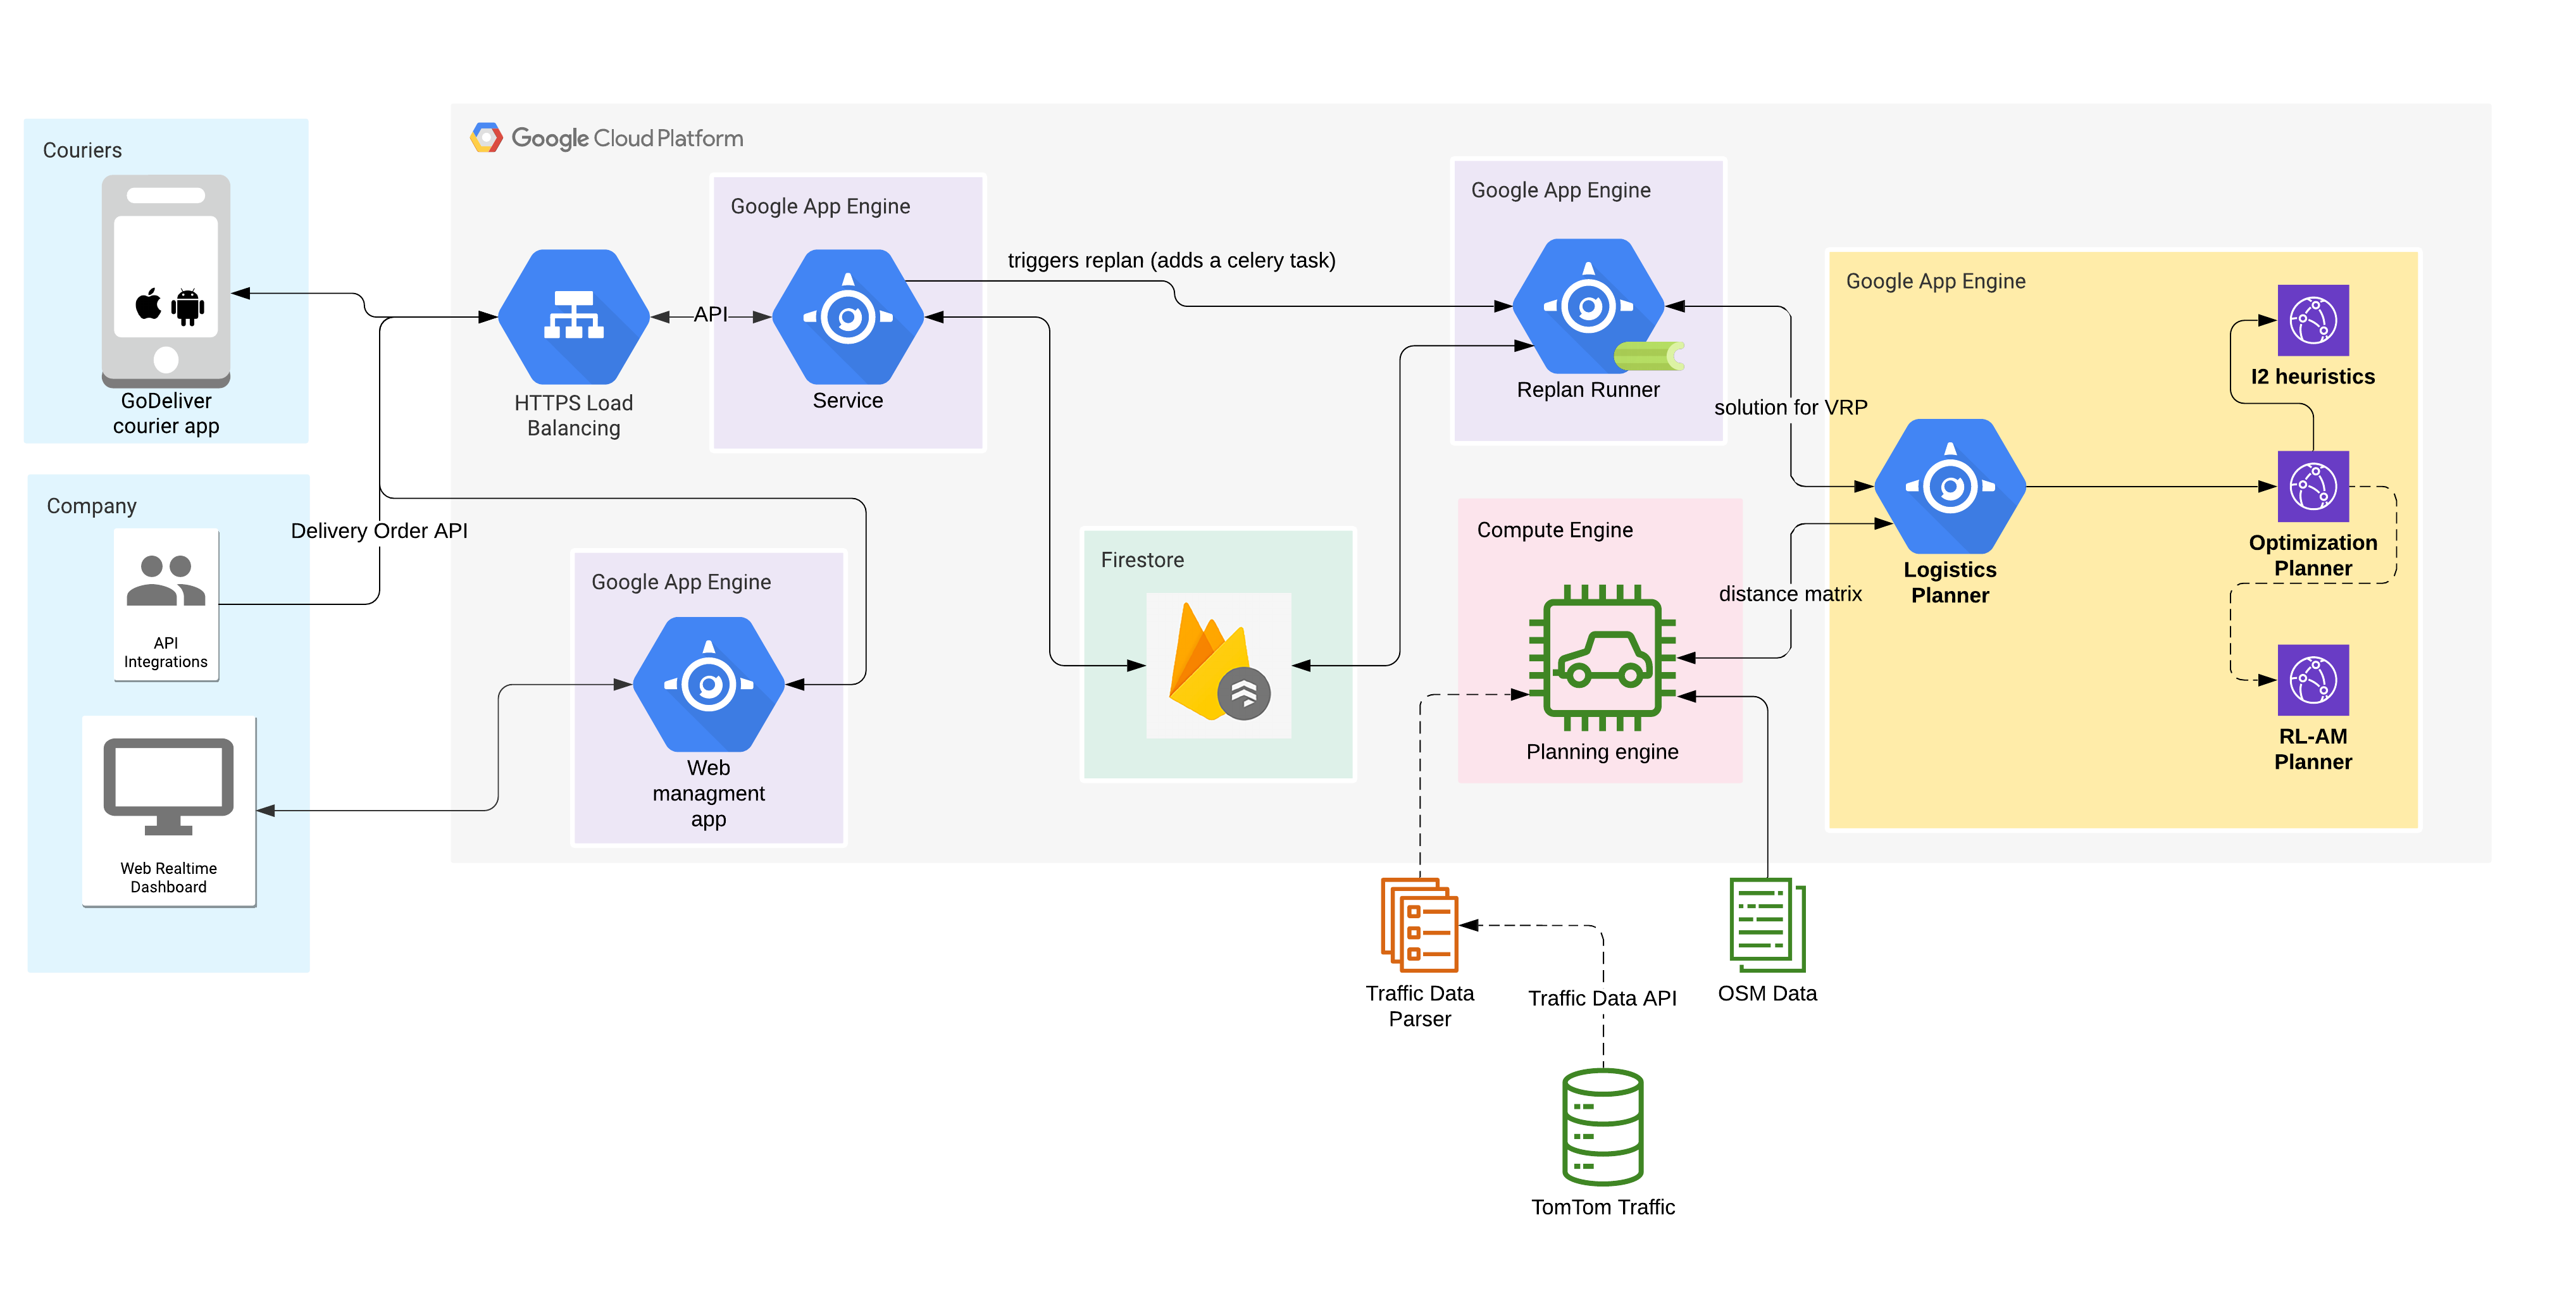
\includegraphics[width=1.0\textwidth]{resources/implementation/godeliver-system.png}
    \caption{GoDeliver System Architecture}
    \label{fig:godeliver-system}
\end{figure}

\subsection{Planning process}
The planning process is a complex operation which requires to work asynchronously because the planning of delivery orders is a time-consuming operation. The modern delivery planners have to support dynamic rescheduling and autonomously act upon the constantly changing environment.

The first part of the planning process is the creation of a delivery order, which is a request for delivery via API. The delivery order is saved in the database by GoDeliver Service with additional meta-data about the delivery state, etc. The database is monitored for a so-called \textit{trigger changes} which fires a replanning job via a distributed task queue Celery. The \textit{trigger changes} are a list of actions such as creation of a new delivery order, changes in courier capacity, or a significant delay of delivery.

If such a replanning job is created, it is saved in Celery queue which processed by GoDeliver Replanning Service. The replanning service loads a business configuration, delivery orders, and delivery plans from the database. It transforms the data into a generic structure which is accepted by our another service logistics planners that are solving the vehicle routing problem. The generic plan structure for the logistics planner freezes some delivery points which should not be considered by the planner since we do not want to change the current in-progress delivery points. This process is enabling us to perform the dynamic vehicle routing problem \ref{dynamic}.

Based on the business config, the desired vehicle routing solver is invoked via the logistics planner API. Usually, the planner takes the previous delivery plan and performs a heuristic algorithm like insertion heuristic which outputs an extended feasible plan. This plan is then improved by a local search algorithm to improve its cost function. Then the solution is processed by GoDeliver Replanning Service and saves the new delivery plans into the database.

In the future, the proposed \gls{vrptw} \gls{ai} planner will be used instead of insertion heuristics because we expect the \gls{ai} planner will outperform the insertion heuristics. The downside is that \gls{ai} planner is not able to leverage on the previous solution, which can lead to drastic changes in the solution structure of the delivery plan. However, this side effect is not a blocker since couriers only see one current delivery point from the delivery plan via GoDeliver mobile app \ref{fig:godeliver-app}.

\begin{figure}[ht]
    \centering
    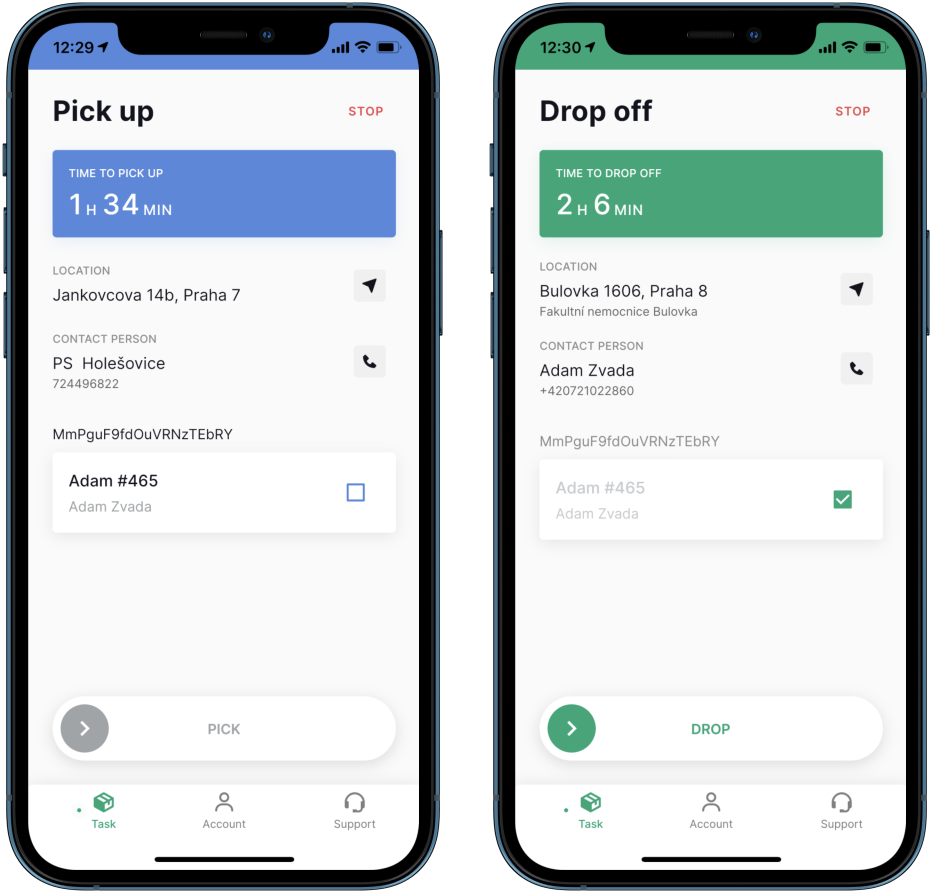
\includegraphics[width=0.25\textwidth]{resources/implementation/godeliver-app.png}
    \caption{GoDeliver Driver App}
    \label{fig:godeliver-app}
\end{figure}

\subsection{Planning Requirements}


\section{VRPTW via Optimization}

\section{VRPTW via AI}